\chapter{Experimental Results}

%TODO: Say how do we update the model (just for three iteration) with Bellman equation
%TODO: say we use MaxQ for model based approach

\section{Planning with Static Assumptions}
\label{se:Model}

Based on the results of the previous section, we can safely use any approximate model-based method 
to learn the Q-values of subtasks which do not belong to $TC(H)$ without worrying
that it will violate the optimality condition. Model-based RL requires the enumeration of all possible states during the planning process.
However, it is not feasible when the state space is too large.
Previous methods (\cite{ApproxDyna, ApproxTree}) rely on function approximation
techniques to predict the next state. Their model is biased because it is possible 
to encounter different next states given the same state and policy for a stochastic problem. If we 
predict one of them, we ignore the stochastic nature of the problem. If we predict
several, the number of states under consideration may grow exponentially with the number of simulating steps
and become intractable after a few steps.

We notice that, for some applications, there are some variables which are more important
than others. Take the mobile robot navigation problem, for example; the location of the robot 
is the key to the planning process, while the movement of other objects in the environment is less important.
Our idea is to separate the variables into planning variables 
and environment variables. During the planning process, we enumerate all possible values of the planning variables, while assuming 
the remaining environment variables are static throughout the process. 
If we limit the number of planning variables to be small, the enumeration process can be efficient.
It also simplifies the learning of the transition and reward functions, since we only need to learn
the dynamics and reward models for the planning variables.

Let state $s = (x, y)$, where $x$ consists of planning variables and $y$ consists of environment
variables. Following the MAXQ approach, we decompose the Q-function as:
\begin{equation}
    Q^{\pi}(i, x, j) = Q_r^{\pi}(i, x, j) + Q_c^{\pi}(i, x, j),
    \label{eq:biasedMaxQ}
\end{equation}
where $Q_r^{\pi}(i, x, j)$ is provided by the child subtask $M_j$.

The task of subtask $M_i$ is to compute $Q_c^{\pi}(i, x, j)$ by:
\begin{equation}
    Q_c^{\pi}(i, x, j) = \sum_{x'} P_m^{\pi}(x'|s, j)[Q_r^{\pi}(i, x', \pi_i(x')) + Q_c^{\pi}(i, x', \pi(x'))],
    \label{eq:biasedQc}
\end{equation}

With the formula above, the Q-values can be computed by dynamic programming.

For simplicity, we use the multi-time model \cite{SMDP} to model the transition function: 
\begin{equation}
    P_m(x|s, j) = \sum^{\infty}_{N=1} \gamma^N P(x, N|s, j).
    \label{eq:multiProb}
\end{equation}

$P_m(x|s, j)$ can be estimated by:
\begin{equation}
    \tilde{P}_m(x|s, j) = (1-\alpha)\tilde{P}_m(x|s, j) + \alpha [ \gamma^N \delta_{x'x}],
    \label{eq:approxP}
\end{equation}
for all $x \in S_i$, where $\delta_{x'x}=1$ if $x' = x$ and is 0 otherwise.
\section{Bus Domain}
\begin{figure}[t]
%\begin{center}
 \begin{minipage}[b]{0.5\linewidth}
    \begin{center}
    %\includegraphics[height=11em, width=6em]{eli_bend.eps}
    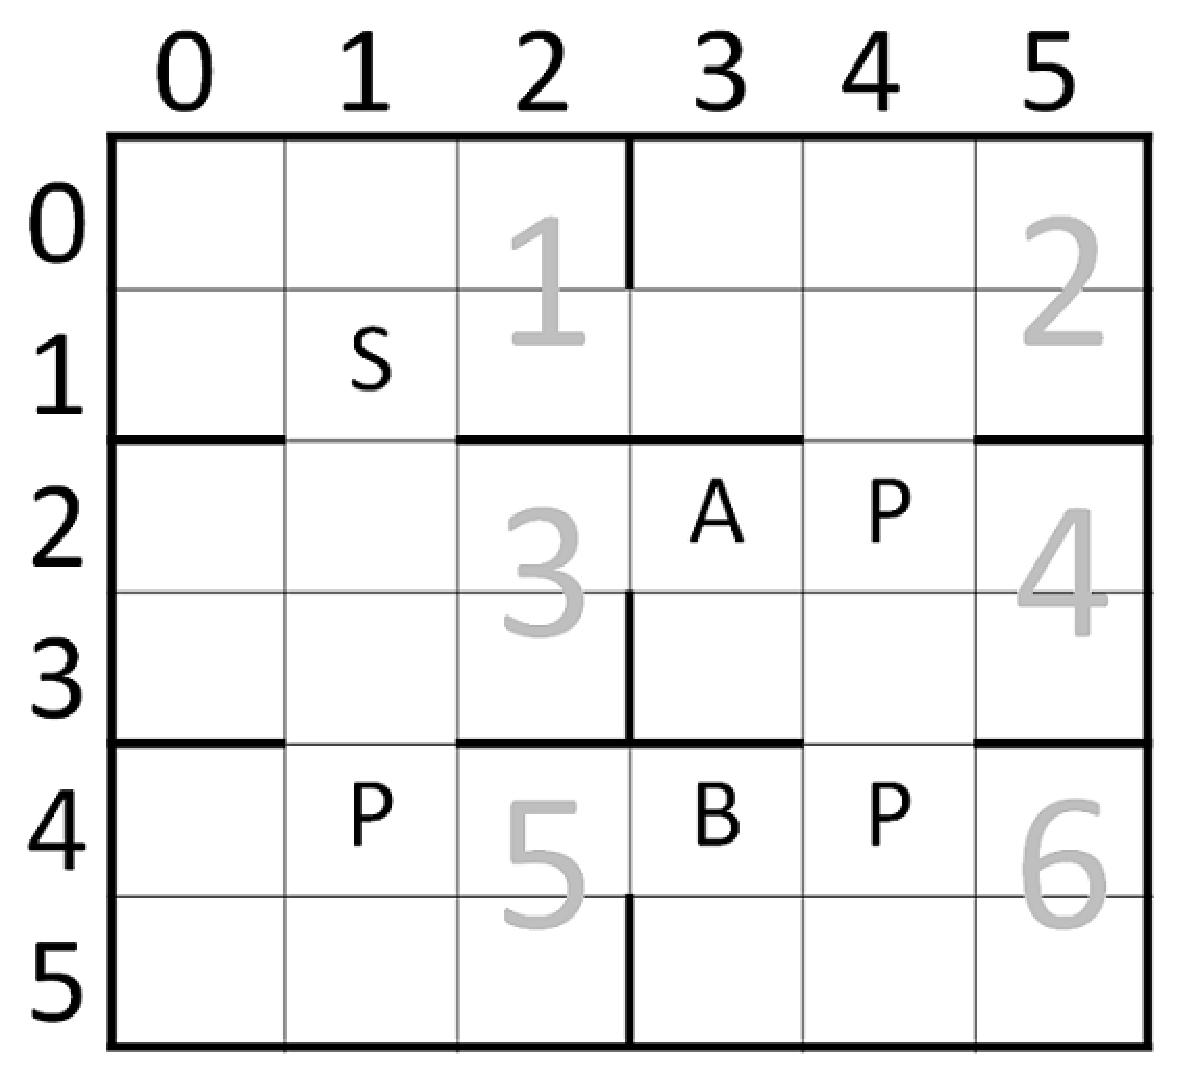
\includegraphics[width=2.0in] {./figures/BusSmall.eps}
    %\caption{(a)}
\end{center}
\end{minipage}
\begin{minipage}[b]{0.5\linewidth}
    \begin{center}
    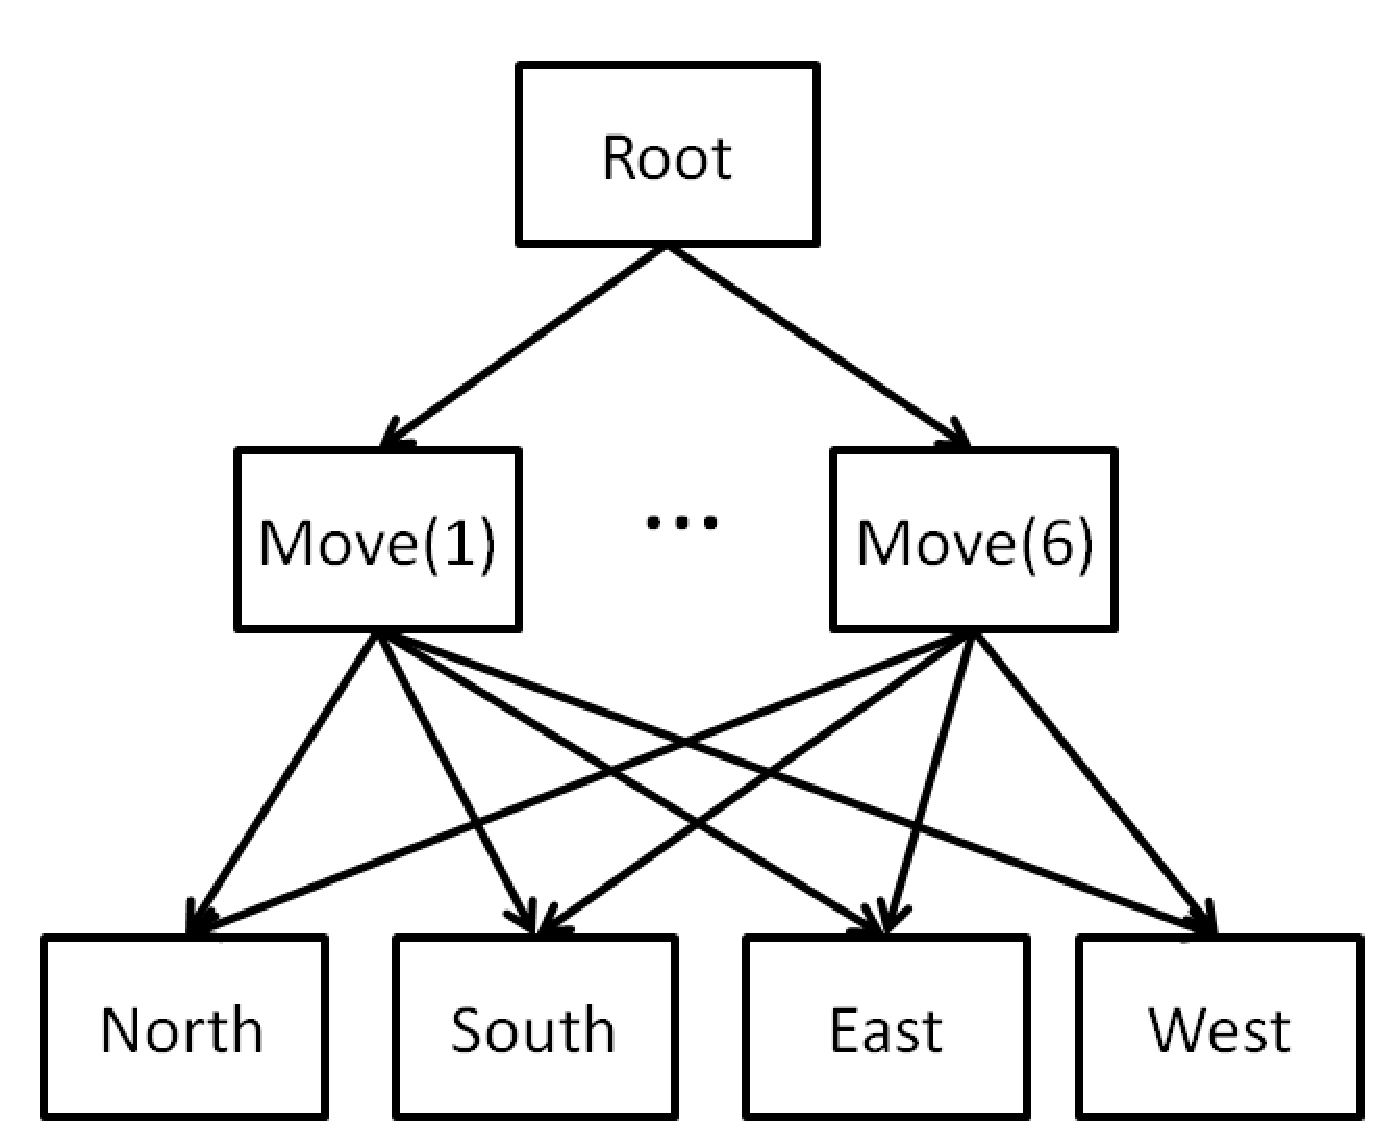
\includegraphics[width=2.0in] {./figures/BusHierarchy.eps}
\end{center}
\end{minipage}
\begin{minipage}[b]{0.5\linewidth} \centering (a) \end{minipage}
\begin{minipage}[b]{0.5\linewidth} \centering (b) \end{minipage}

%\end{center}
\caption{(a) The school bus domain (b) A task graph for the school bus domain.}
\label{fig:bus}
\end{figure}

Figure \ref{fig:bus}(a) shows the school bus domain. The school bus starts at school $S$. Its task 
is to pickup all passengers marked as $P$ and return to the school.
The bus can move North, South, East, or West. There is a reward of -1 applied for each action.
There is 0.1 probability for the bus to move in a random direction. It stays put 
when trying to cross a wall. 
The passengers are picked up automatically when the bus moves into
the location of a passenger. The passengers can be picked up in any order.
The episode ends when it finishes the task.  
There are two possible locations for road construction. They are marked as 
$A$ and $B$. If the bus passes a construction site, it will get damaged with probability 1 and has the probability
of 0.25 to break down for each step afterwards. There is a reward of -50 if the bus breaks down and the episode ends immediately. 
At the beginning of an episode, the status of the road is randomly chosen from no construction, $A$ is under construction,
or $B$ is under construction. There is a 0.05 probability for the road status to change after the episode begins.
The world is divided into six areas. There are six subtasks $Move(1), \dots,$ and $Move(6)$ which move the
bus to the corresponding area.
Subtask $Move(t)$ can only be invoked if $t$ is the adjacent area.
The subtask terminates if the bus exits the current area.
When it terminates, a pseudo-reward $\tilde{r}$ is applied if the bus arrives at designated area $t$ and 0 otherwise.
The task hierarchy is shown in Figure \ref{fig:bus}(b). 

A state can be described by the 8-tuple $(x, y, h, p_1, p_2, p_3, a, b)$, where $(x, y)$ is the location of 
bus, $h$ shows if the bus is damaged, $p_i$ indicates if the corresponding passenger has been picked up or not,
and $a$ and $b$ are binary variables which indicate the status of the construction sites.
The planning variables of our model are $\{x, y, p_1, p_2, p_3\}$, while the damage
status and road conditions are assumed to be static during the planning process.
Our model can learn that a large penalty will be received when the bus is damaged.  
%Since the damage status is assumed static during the planning process, 
However, our model cannot learn that the bus will get damaged if it passes through
a construction site. The model is certainly biased in this case, thus
it cannot learn the optimal policy. The objective of 
the experiment is to show that the optimal policy can still be learned
if we combine the model-based approach with HORDQ. 

Since the six subtasks $Move(1), \dots,$ and $Move(6)$ cover all primitive actions, they form a total leaf cover of the hierarchy.
We used HORDQ in the subtasks to guarantee the convergence to the optimal
policy. Subtask $Root$ adopted our approximate model-based method. 

%The planning variables include 
%the location of bus and the status of passengers. The environment variables are the 
%damage status of bus and the status of road. 
%TODO: total leaf cover always exist
%The world is divided by 6 areas. 

\begin{figure}[t]
%\begin{center}
 \begin{minipage}[b]{0.5\linewidth}
     \begin{center}
    %\includegraphics[height=11em, width=6em]{eli_bend.eps}
    \includegraphics[width=2.5in] {./figures/Approx.eps}
\end{center}
    %\caption{(a)}
\end{minipage}
\begin{minipage}[b]{0.5\linewidth}
     \begin{center}
    \includegraphics[width=2.5in] {./figures/Random.eps}
\end{center}
\end{minipage}
\begin{minipage}[b]{0.5\linewidth} \centering (a) \end{minipage}
\begin{minipage}[b]{0.5\linewidth} \centering (b) \end{minipage}

%\end{center}
\caption{The learning curve for the school bus domain, averaged over 400 episodes. (a) With our model-based approach. (b) With random planner.
The pseudo-reward is shown in parentheses. The parameters are $\alpha=0.1$ and $\gamma=1$. All algorithms follow an $\epsilon$-greedy exploration policy
with $\epsilon = 0.1$.}
\label{fig:res}
\end{figure}

Figure \ref{fig:res}(a) shows the learning curves with different level of pseudo-rewards.
With pseudo-reward +60, it learned a suboptimal policy because
the pseudo-reward is too large to make subtask $Move(t)$ ignore 
the penalty of breakdown. As a result, the subtask followed 
the instruction of its parent too strictly.

On the other hand, if we do not impose any pseudo-reward, 
the optimal policy can be learned, but the learning rate is
slower than SARSA(0) learning. Since the subtask has no
incentive to follow the instruction from the hierarchy, 
the learning process is similar to SARSA(0) learning 
except it has six different Q-functions to learn (one for each subtask) instead of one.
Thus it takes longer to learn the optimal policy. 

With the appropriate pseudo-reward, we can get a near-optimal policy
while the learning rate is faster than SARSA(0)
Our experiment shows that a pseudo-reward of +5 is enough to make the subtask follow 
the order of $Root$ in most of the times, but it is not enough for the subtask to ignore
the breakdown penalty. For example, when $Root$ executes $Move(4)$ to move the bus from area 
3 to area 4 and the road at location $A$ is under construction, $Move(4)$ subtask
will learn it is a bad decision with HORDQ.
Instead of moving to area 4, $Move(4)$ may move to area 1 or 5 to avoid
the breakdown penalty. In turn, $Root$ learns $Move(4)$ cannot be executed in 
such a scenario, thus it will seek an alternate plan if the same scenario
is encountered.

To illustrate the undesirable result when some suboptimal subtasks exist in 
the hierarchy and the MAXQ framework is adopted, we combine our approximate model-based approach
and MAXQ-Q learning in our experiment. The combination learns a suboptimal policy similar to HORDQ with high pseudo-reward. 
Since MAXQ does not estimate the consequence of its action outside its own subtask,
$Move(t)$ will move to area $t$ at any cost. It leads to the frequent damage of the school bus.

To simulate the performance of the combination of a poorly-approximated model-based method and 
HORDQ, we replaced our model-based approach with a random policy.
The result is shown in Figure \ref{fig:res}(b). In this case, SARSA(0) has the fastest
learning rate. It takes more time for $Move(t)$ to realize that the policy of $Root$ is bad with higher pseudo rewards.
Nevertheless, it will eventually learn a near-optimal policy.
The combination of random policy and MAXQ has the worst result.

The result shows that a good approximate model 
can help increase the learning rate with the combination of HORDQ. 
If the model is poor, HORDQ serves as a fail-safe mechanism to stop 
the agent repeating the same poor policy over and over again.
On the other hand, MAXQ learned a poor policy in both cases.  
The result suggests that in order to construct a robust HRL 
algorithm, it is beneficial to incorporate HORDQ in the hierarchy.

%On the contrary, the combination of MAXQ and a poor approximated model has
%a performance similar to random policy.

%TODO: add random agent experiment
%TODO: if I set the pseudo reward to zero, will the whole stuff breaks down again?


\section{Super Mario Brothers}

%reward system here
%and pseudo reward
\subsection{Planner}
We adopt our static assumption on all objects except Mario. The state of Mario 
can be described by a 4-tuple $(x, y, dx, dy)$, where are the location and speed of Mario. 
The ranges of $x$, $y$, $dx$ and $dy$ are $[0, 21]$, $[0, 15]$, $[-2, 2]$, and $[-2, 2]$.
These variable are continuous, so it is not possible to enumerate all possible states
of Mario. It is possible to discretize the variables, but the resulting state space 
is still too large if we want to predict the dynamics of Mario in fine detail.
It makes it impossible to adapt the dynamic programming technique to Super Mario Bros.

Instead of enumerating all possible states of Mario, the planner in our experiment 
is a $K$-step lookahead greedy search algorithm. The planner searches the states
which can be reached from the current state within $K$ steps and returns a sequence of
steps which achieve the highest reward.

%details
In our experiment, we do not assume the planner has the prior knowledge about 
the dynamics of Super Mario Bros. To learn the dynamics of Mario, we use regression trees
to predict the future position and speed of Mario. 
The features are represented by the speed of Mario and the tiles within 5 by 5 
area around Mario. There are 27 variables. 
Since each action has different dynamics, 
We build different trees for different actions. 
Given the current state and action, the regression trees should predict 
the x-speed and y-speed of the following state. It is possible to predict
the next x-position and y-position of Mario, but 
it can be more generalizable if we predict difference of the positions $\epsilon_x = x' - x$ and 
$\epsilon_y = y' - y$. The 4 variables are the class variables for the regression trees.
For simplicity, we separately build regression trees for different class variables. 
In our current implementation, there are 9 actions and 4 class variables, so we 
have 36 regression trees to model the dynamics of Mario. 

It is crucial for the planning process to learn when Mario is going to be killed. 
However, the number of samples right before Mario getting killed is limited by the
number of episodes, which is much smaller than the number of steps. 
To efficiently use the available samples, we use a single regression tree to learn the 
reward function.

%lookahead planning
We adopt greedy search in our planning process.
The planning process begins with a state of Mario. 
Then it iteratively acquires the next states by applying
the 9 actions to the state. To avoid fully expand the whole search tree to 
the depth $K$, which is time-consuming and unnecessary, we expand the state
with the largest predicted reward. 
The process stops after we acquire $M$ nodes, then the planner returns 
a sequence of actions which achieves the highest predicted reward.
Since we may not search the tree fully, it is possible to have 


%TODO: add model the difference here (Peter's paper)
%

\subsection{}
\endinput
%Most of the previous work on RL focus on model-free approaches for several reasons. 
%The most 
%Within a planning agent, there are at least two roles for real experience: it
%can be used to improve the model (to make it more accurately match the real
%environment) and it can be used to directly improve the value function and
%policy using the kinds of reinforcement learning methods we have discussed in
%previous chapters. The former we call model-learning, and the latter we call
%direct reinforcement learning (direct RL). The possible relationships between
%experience, model, values, and policy are summarized in Figure  9.2. Each arrow
%shows a relationship of influence and presumed improvement. Note how experience
%can improve value and policy functions either directly or indirectly via the
%model. It is the latter, which is sometimes called indirect reinforcement
%learning, that is involved in planning. 

%The second branch is model-based RL, which directly estimates
%a model of the environment and then plans with
%this model. Early work demonstrated that summarizing an
%agent’s experience into a model could be an efficient way
%to reuse data (Moore & Atkeson, 1993), and later work utilized
%the uncertainty in an agent’s model to guide exploration,
%yielding the first (probabilistic) finite bounds on the amount of data required
%to learn near-optimal behaviors in the general case (Kearns & Singh, 1998;
%Kakade, 2003).


%motivation: play a randomly generate maze to adapt to
%adapt to noval situation

%weakness-> an adversary to block the path forever
%no knowledge (coin won't disappear-->need hack to do it, moster won't move)
%comparison to the previous work->HRL,


%model based-> state space is too large. good to train with
%few examples (10 sec training)
%model free-> cannot handle randomly generated maze -> failed to adapt to noval situation. can handle large space (linear SARSA)
%Experiment: comparison with flat model based approach and hierarchical model based approach with approximation

%combine both-> use model based on top level to reduce
%the state space, and model free on bottom to 
%deal with randomized noisy world for short term reward

%build multilevel of hierachy on features
%label each room with a number 1, 2, 3
%the coordinate of wrt the room
%(1, (25, 30))
%move from room 1 to room 2
%top level
%action (1->2)
%second level
%assume (1, (25, 30)) -> (2, (0, 0))
%action ((25, 30) -> (0, 0)) goal (-25, -30) in single step

%need to build time model of the full state
%P(s->s'|x, t) the propability to move from state s to s'
%after t steps of the observation of full state x

%power coms from trasition model (model the shortest path), not shortest path
%you can use model-based approach on this

%fickle passenger of MaxQ
%coarseness on time and space scale

%-->you can work on continus varible now, no more grid world

%1. Assumption on the state difference (if it is not true --> like the agent in a world boundary or the health is 100 and cannot be imporve
  %since the state is outside the known state boundary, the planner whon't plan for it. but the local planner may still direct the agent
  %to go outside the world boundary, which may be a problem)
%2. Application to the hierachical RL
%3. Limitation: unachievable state (a coin surrounded by many monsters)
%4. Can inference in a very small world, not need to do 64 by 64
%Sometimes we need a plan. The greedy approach of reinforcement learning does not always work. 
%RL techniques have several limitations:
%1. It's difficult for to transfer the value function from a small world to a large one. If the agent has
%the experience only in a small world like 4 \times 4 grid, it cannot act well in 64 \times 64 grid
%because it does not know the correct action in regard to an object 63 grid away.

%2. It takes a long time to train the agent to be good enough. The greedy 

%3. The approximation only good in a small range. We need a plan for long term action.
%The noval state (the state in current game which has not been experienced) may 

%4. Impossible task to maze problems: RL require that optimal agent to find the optimal solution for a maze when all the features
%are input to the agent. Which is unlikely to work.(impractical when the maze is large)(unable to transfer
%the knowledge from previous maze experience to the current one) A practical solver shall invovle planning through 
%the possible route and find the one which can lead to the exist.
%All the work requires the agent to repeat play the same maze (assuming traps) until it finds the optimal solution.
%What if the maze changes every time?

%1. Is it guarranteed convergence? Yes, if we choose the goal next to the current state which leads to highest Q value. 
%It is the same as SARSA.
%2. How to choose the goal to guarrante convergence to optimal policy?

%Good to work on the problem with a long term reinforcement (feedback) like a maze.
%Bad to work with a problem with dynamic envirment (everything changes with or without agents actions)
%Bad when the consequence of an action is delayed for many steps. (poison)

%Q: prove that RL cannot solve maze problem
%Ability to transfer the knowledge from one maze to another
%compare the HRL in key-finding problem
%compare to the model-based RL





%application: the key-room problem--> each room lock a key, one room has a treasure, the agent needs to go through 
%a maze to collect the keys for each door and get the treasure

%Stochastic Shortest-Path Problems
%A Stochastic Shortest-Path problem is an mdp prob-
%lem in which the state space S = f1; : : : ; n; tg is such
%that t is a goal (target) state that is absorbing (i.e.,
%p(t; u; t) = 1 and g(t; u) = 0 for all u 2 U(t)), and the
%discount factor ® = 1. In this case, the existence of
%optimal policies (and optimal stationary policies) is a
%major mathematical problem. However, the existence
%is guarantee under the following reasonable conditions:
%(A1) There exists a policy that achieves the goal with
%probability 1 from any starting state.
%(A2) All costs are positive.
%The ¯rst assumption just expresses the fact that the
%problem admits a well-behaved solution. Such policies
%are known as proper policies. The second assumption,
%in the other hand, guarantees that all improper policies
%incurs in in¯nite cost for at least one state. Thus, both
%assumptions preclude cases where the optimal solution
%might \wander" around without never getting to the
%goal. For example, a problem having a zero-cost cycle
%(in state space) violates the second assumption.
%As mentioned in the Introduction, often we are only
%interested in knowing how to go from a ¯xed initial
%state, say 1, to the goal state. The optimal solution in
%this case is an partial optimal stationary policy ¹ such
%that ¹(i) = ¹¤(i) for all states i that are reachable
%from 1 when using the optimal policy ¹¤; the so-called
%relevant states when starting from 1.1
%Finding a partial optimal policy can be consider-
%ably simpler, the extreme case when the set of relevant
%states is ¯nite and the complete state space is in¯nite.
%Thus, the question of how to ¯nd partial optimal poli-
%cies is of great relevance. One algorithm for that is
%Real-Time Dynamic Programming.

%There are two ways for a RL agent to use its sample data. It can use the sample data to update the 
%value function and improve its policy. It is called model-free (or direct) reinforcement learning. 
%Another approach is to use the sample data to estimate parameters for the model of the environment and compute the value function
%from the model. It is called model-based (indirect) reinforcement learning.

%The advantage of model-based approaches is that they make more efficient use of the sample data, thus 
%it take fewer time to train a model-based RL agent. Other the other hand, model-free approaches do not assume 
%a prior model, so it would not be affected by the bias of the model design. Besides, the existence of 
%good linear approximation algorithms, such as linear SARSA, makes it possible for model-free approaches to
%handle large scale problems.

%Model-based approaches needs to enumerate through all possible states to compute the value function. 
%But the number of states grows exponentially with the number of features, 
%and it quickly becomes intractable if the number features grows large.

%The main idea of this work is to combine the model-free, model-based and hierarchical reinforcement learning.
%For the lower level of hierarchy, we adopt the model-free approach to handle the complete and possibly large state space.
%On the top level of hierarchy, we use the model-based to plan on a coarser level, which contains only small number of states.
%This approach allows the agent to plan on the higher level and make efficient use of the sample data. On the lower level,
%the agent uses model-free approaches with linear approximation to handle the complete state space.

%The prior works on hierarchical reinforcement learning (HRL) can be divided into two categories: model-free and model-based approaches. 
%The model-free approaches include HAMQ \cite{HAMQ}, MAXQ \cite{MAXQ}, SMDP and options framework \cite{option}
%For model-based approaches, Seri et al. \cite{HLearning} proposed a model-based HRL in average reward setting.
%Diuk et al. \cite{Diuk} adopted model-based HRL to deterministic domain. Jong and Stone \cite{RMaxQ} combined 
%R-MAXQ and MAXQ to achieve efficient model-based exploration and the action abstraction of MAXQ.

%TODO: show that model based state difference can learn randomly generated maze with very limited steps (only four touches of the wall)
%TODO: use a poison example to show the limit of pure approximated model-based approach and the motivation
%of use hierarchical optimal policy for pseudo reward and recursive optimal policy for real reward. It can be shown that
%it will converge to optimal policy if the true goal state of the game is included as a subgoal(
%the worst case is the child node finish the game by itself)
